Prior to 1940, there were no hints regarding the underlying mechanism of a neuron
as only extracellular recordings were availble. At that time it was known that:
\begin{enumerate}
    \item The cell membranes separes solutions with different ionic concentrations.
    \item \([\text{K}^{+}]_{o}<<[\text{K}^{+}]_{i}\)
    \item \([\text{Na}^{+}]_{o}>>[\text{Na}^{+}]_{i}\)
\end{enumerate}
Moreover, the neuronal activity was believed to be a breakdown of the membrane resistance.\\
Then, the voltage clamp technique was introduced, enabling to maintain the membrane
voltage \(V_{m}\) at any desired level. Thus, it allowed, together with chemical stimulation,
to study the effect of each kind of ion via a selective analysis of the single ionic currents.
As a matter of fact, it was observed that both Na\({}^{+}\) and K\({}^{+}\) ions make significant
contributions to the ionic current underlying the action potential. Therefore, there are changes
in the membrane permeabilities for a few different ions, not for all ions, as thought before.\\
In particular, the action potential amplitude crtically depends on the external concentration of
Na\({}^{+}\) ions.\\
In the classical patch-clamp technique, scientists were able to analyse a patch of cellular membrane
and selectively block some kinds of channels, studying how the behaviour of the remaining ones would
affect the \(V_{m}\) voltage. However, Neher and Sakmann improved such a technique and allowed to
measure the effect on \(V_{m}\) of a single ion channel.\\
Hence, the big remaining question investigated by Hodgkin and Huxley was how the permeability of the
membrane to specific ions is linked to \(V_{m}\) and time. The two researchers managed to
disentangle the temporal contributions of different ions assuming that they responded
differently to changes in \(V_{m}\).
\begin{figure}[H]
    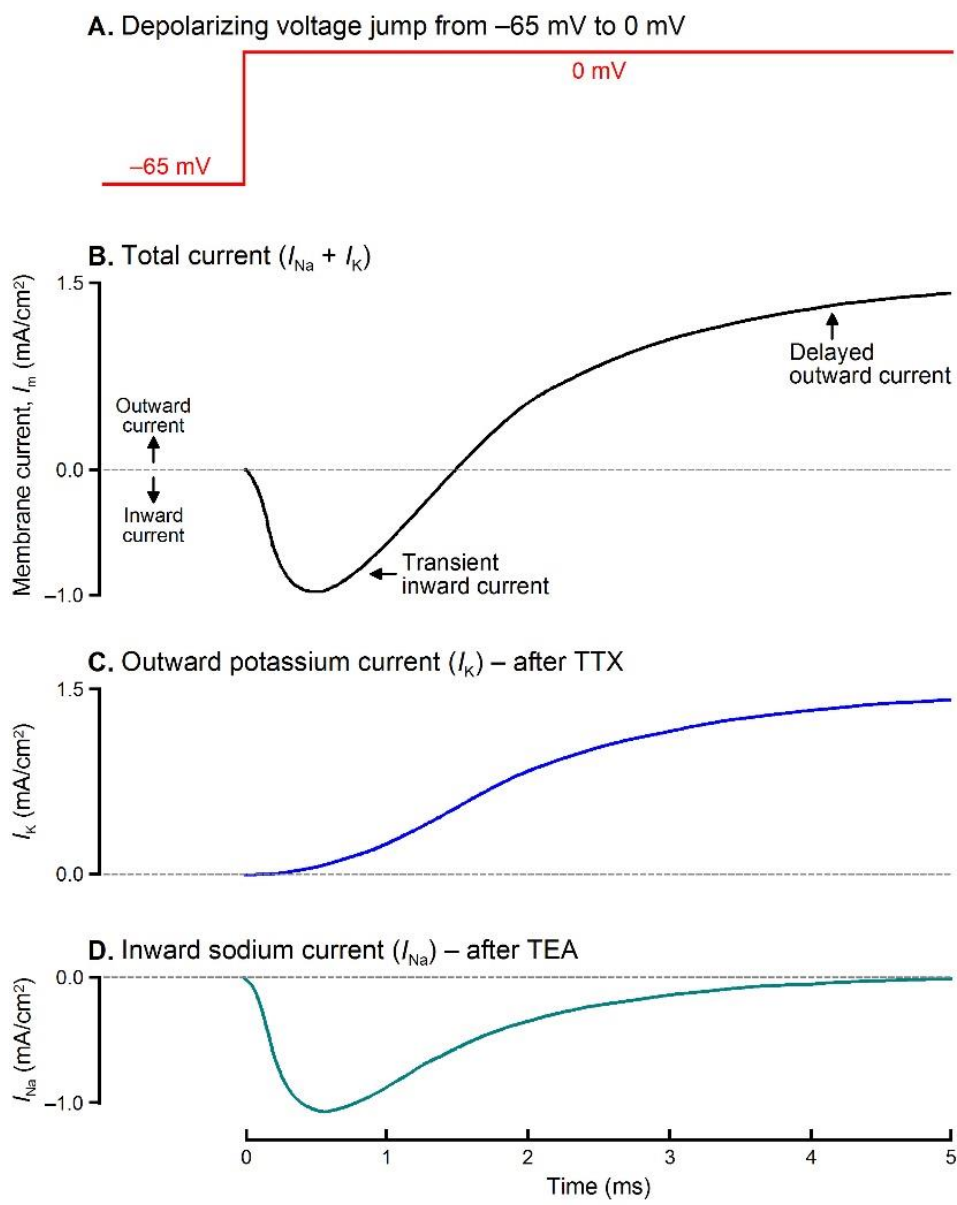
\includegraphics[scale=0.33]{05_1}
    \centering
\end{figure}

\subsection{Equivalent Circuit}
The following equivalent may be used to model virtually any cellular membrane, in particular it
can describe a neuron membrane if the proper ionic channels - i.e., Na\({}^{+}\) and K\({}^{+}\) -
are introduced. Note that also a leakage current \(I_{leak}\) is considered.
\begin{figure}[H]
    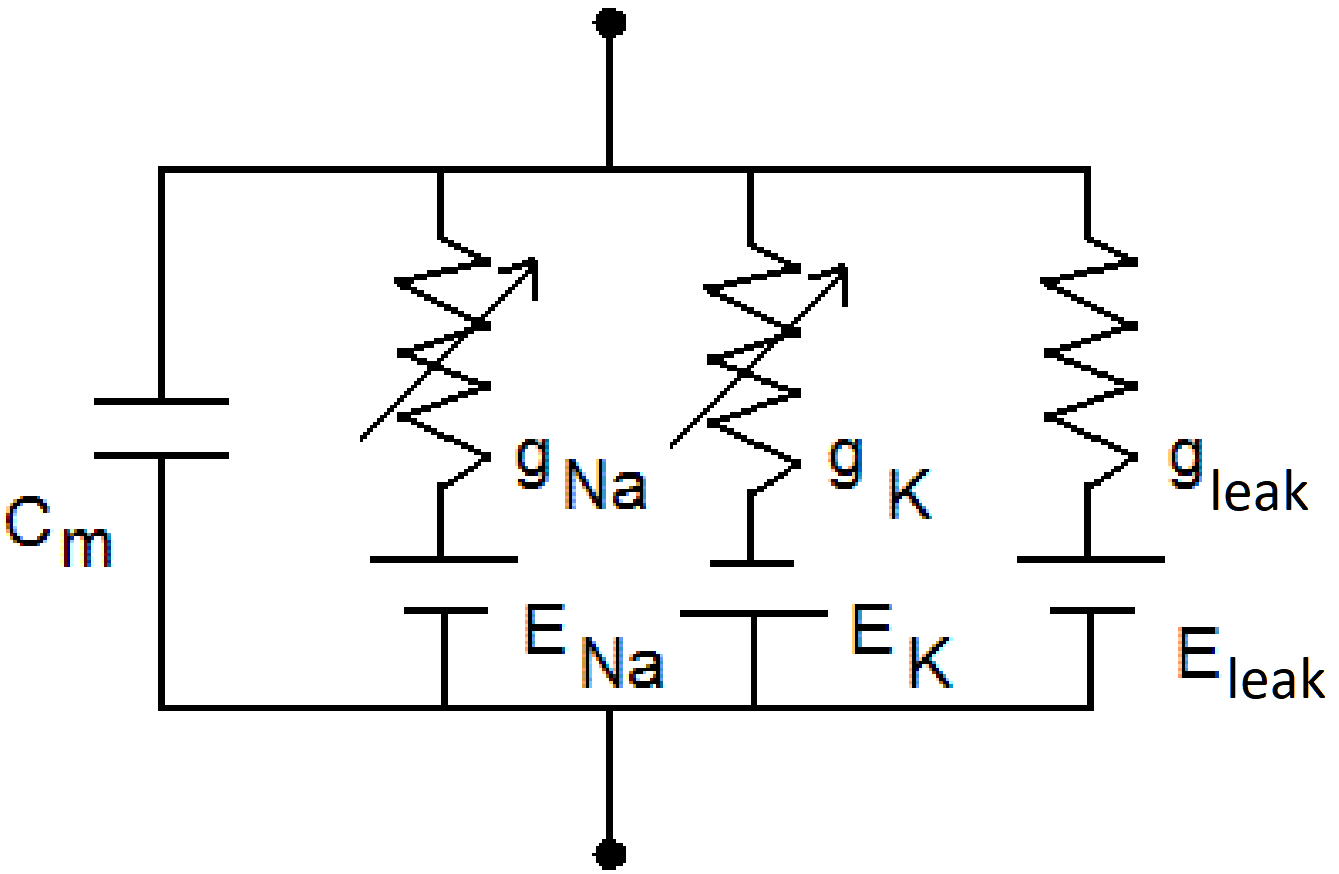
\includegraphics[scale=0.22]{05_2}
    \centering
\end{figure}
Thus, the membrane current is described as:
\begin{equation*}
    I_{m}(t)=I_{ionic}(t)+C_{m}\frac{dV_{m}}{dt}=I_{Na}+I_{K}+I_{leak}+C_{m}\frac{dV_{m}}{dt}
\end{equation*}
Let's now take one of the three ionic current components, for instance Na\({}^{+}\), hence
the sodium current \(I_{Na}\) can be computed thanks to the Ohm's Law:
\begin{equation*}
    I_{Na}(t)=g_{Na}(V_{m}(t),t)\cdot{\bigl[V_{m}(t)-E_{Na}\bigr]}
\end{equation*}
with \(E_{Na}\) being the sodium reversal potential obtained from the Nernst Equation:
\begin{equation*}
    E_{Na}=\frac{RT}{zF}\ln{\frac{[Na]_{o}}{[Na]_{i}}}
\end{equation*}
Therefore, it is clear that sodium and potassium conductances are functions of
both time and membrane voltage, as shown in the image below.
\begin{figure}[H]
    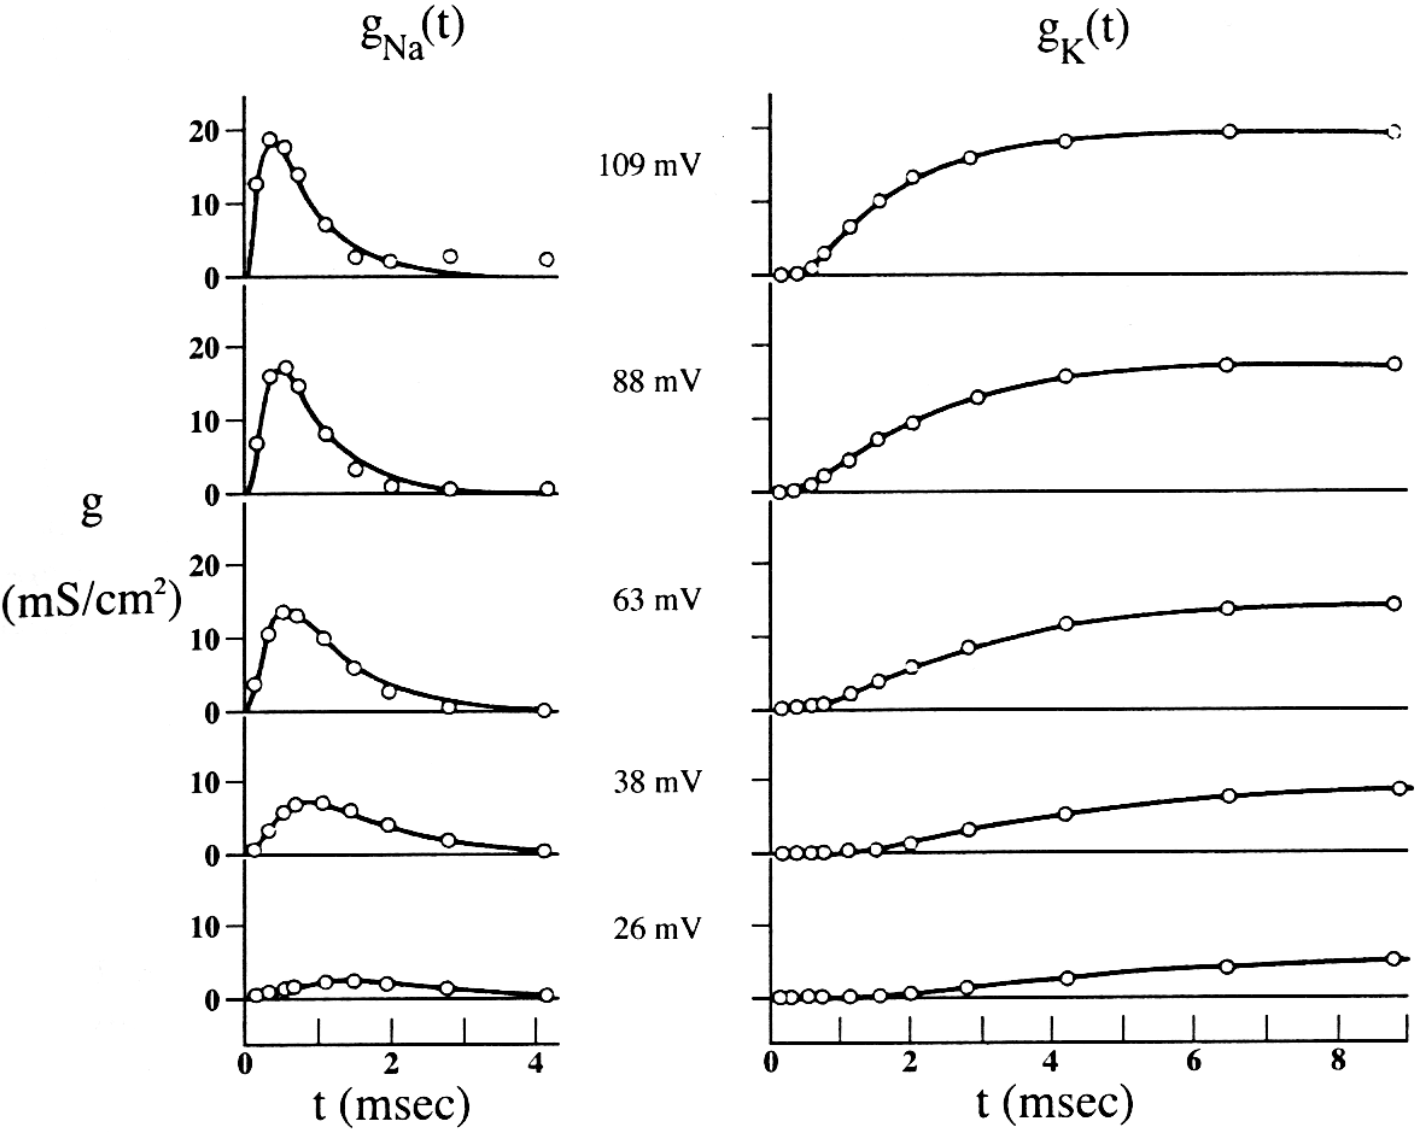
\includegraphics[scale=0.3]{05_3}
    \centering
\end{figure}
Note that the potassium channels dynamics is monophasic - i.e., monotonic - and is delayed
w.r.t. the sodium channels response, in addition it shows no decay.

\subsection{Gating Particles}
The gating particles (\(m\), \(h\), \(n\), \dots) were introduced to describe the dynamics of
the ionic conductances, they can be either activating or inactivating.
\begin{equation*}
    g_{Na}=\bar{g}_{Na}\cdot{m^{3}h}
    \hspace{3cm}
    g_{K}=\bar{g}_{K}\cdot{n^{4}}
\end{equation*}
The sodium kinetics is governed by 2 gating particles, thus its behaviour is biphasic. On the other
hand, the potassium dynamics is monophasic, as it depends only on \(n\).\\
Note that a gating particle \(p_{i}\) value is in the \([0; 1]\) interval and it can be equivalently
seen as the fraction or the probability of gates of type \(i\) being open. On the contrary,
\((1-p_{i})\) represents the fraction of type \(i\) gates being closed.\\
The connection between these two probabilities is governed by two functions:
\(\alpha_{i}(V_{m})\) and \(\beta_{i}(V_{m})\).
Now, this differential equation describing how \(p_{i}\) evolves over time can be derived:
\begin{equation*}
    \frac{dp_{i}}{dt}=\alpha_{i}(V_{m})(1-p_{i})-\beta_{i}(V_{m})p_{i}
\end{equation*}
The steady-state solution \(p_{i_{\infty}}\) is
\begin{equation*}
    p_{i_{\infty}}(V_{m})=\frac{\alpha_{i}(V_{m})}{\alpha_{i}(V_{m})+\beta_{i}(V_{m})}
\end{equation*}
while the time constant for the channels of type \(i\) is
\begin{equation*}
    \tau_{i}(V_{m})=\frac{1}{\alpha_{i}(V_{m})+\beta_{i}(V_{m})}
\end{equation*}
\paragraph{Potassium Current}
\begin{equation*}
    I_{K}=g_{K}(V_{m}-E_{K})=\bar{g}_{K}\cdot{n^{4}}\cdot{(V_{m}-E_{K})}
\end{equation*}
where \(\bar{g}_{K}=36\;mS/cm^{2}\).\\
\(n\) is an \textbf{activating} particle, where the two \(\alpha_{n}\) and \(\beta_{n}\)
functions are:
\begin{equation*}
    \alpha_{n}(V_{m})=\frac{10-V_{m}}{100\cdot\bigl(e^{\frac{10-V_{m}}{10}}-1\bigr)}
    \hspace{3cm}
    \beta_{n}(V_{m})=0.125\cdot{e^{-\frac{V_{m}}{80}}}
\end{equation*}
with \(\alpha_{n}\) being a sigmoidal function and \(\beta_{n}\) an exponential-like function.
Finally, the time-dependent solution can be written as:
\begin{equation*}
    n(t)=n_{\infty}-(n_{\infty}-n_{0})e^{-\frac{t}{\tau_{n}}}
\end{equation*}
\paragraph{Sodium Current}
\begin{equation*}
    I_{Na}=g_{Na}(V_{m}-E_{Na})=\bar{g}_{Na}\cdot{m^{3}h}\cdot{(V_{m}-E_{Na})}
\end{equation*}
where \(\bar{g}_{Na}=120\;mS/cm^{2}\).\\
\(m\) is an \textbf{activating} particle, where the two \(\alpha_{m}\) and \(\beta_{m}\)
functions are:
\begin{equation*}
    \alpha_{m}(V_{m})=\frac{25-V_{m}}{10\cdot\bigl(e^{\frac{25-V_{m}}{10}}-1\bigr)}
    \hspace{3cm}
    \beta_{m}(V_{m})=4\cdot{e^{-\frac{V_{m}}{18}}}
\end{equation*}
\(h\) is an \textbf{inactivating} particle, where the two \(\alpha_{h}\) and \(\beta_{h}\)
functions are:
\begin{equation*}
    \alpha_{h}(V_{m})=0.07\cdot{e^{-\frac{V_{m}}{20}}}
    \hspace{3cm}
    \beta_{h}(V_{m})=\frac{1}{e^{\frac{30-V_{m}}{10}}+1}
\end{equation*}
Finally, the following two plots are derived. The first one depicts the gating particles
time constants vs. the membrane voltage \(V_{m}\) and it can be seen that \(m\) has a
super fast dynamics when compared to the other two particles. The second plot shows
the gating particles activating or inactivating effect as a function of the membrane
voltage \(V_{m}\).
\begin{figure}[H]
    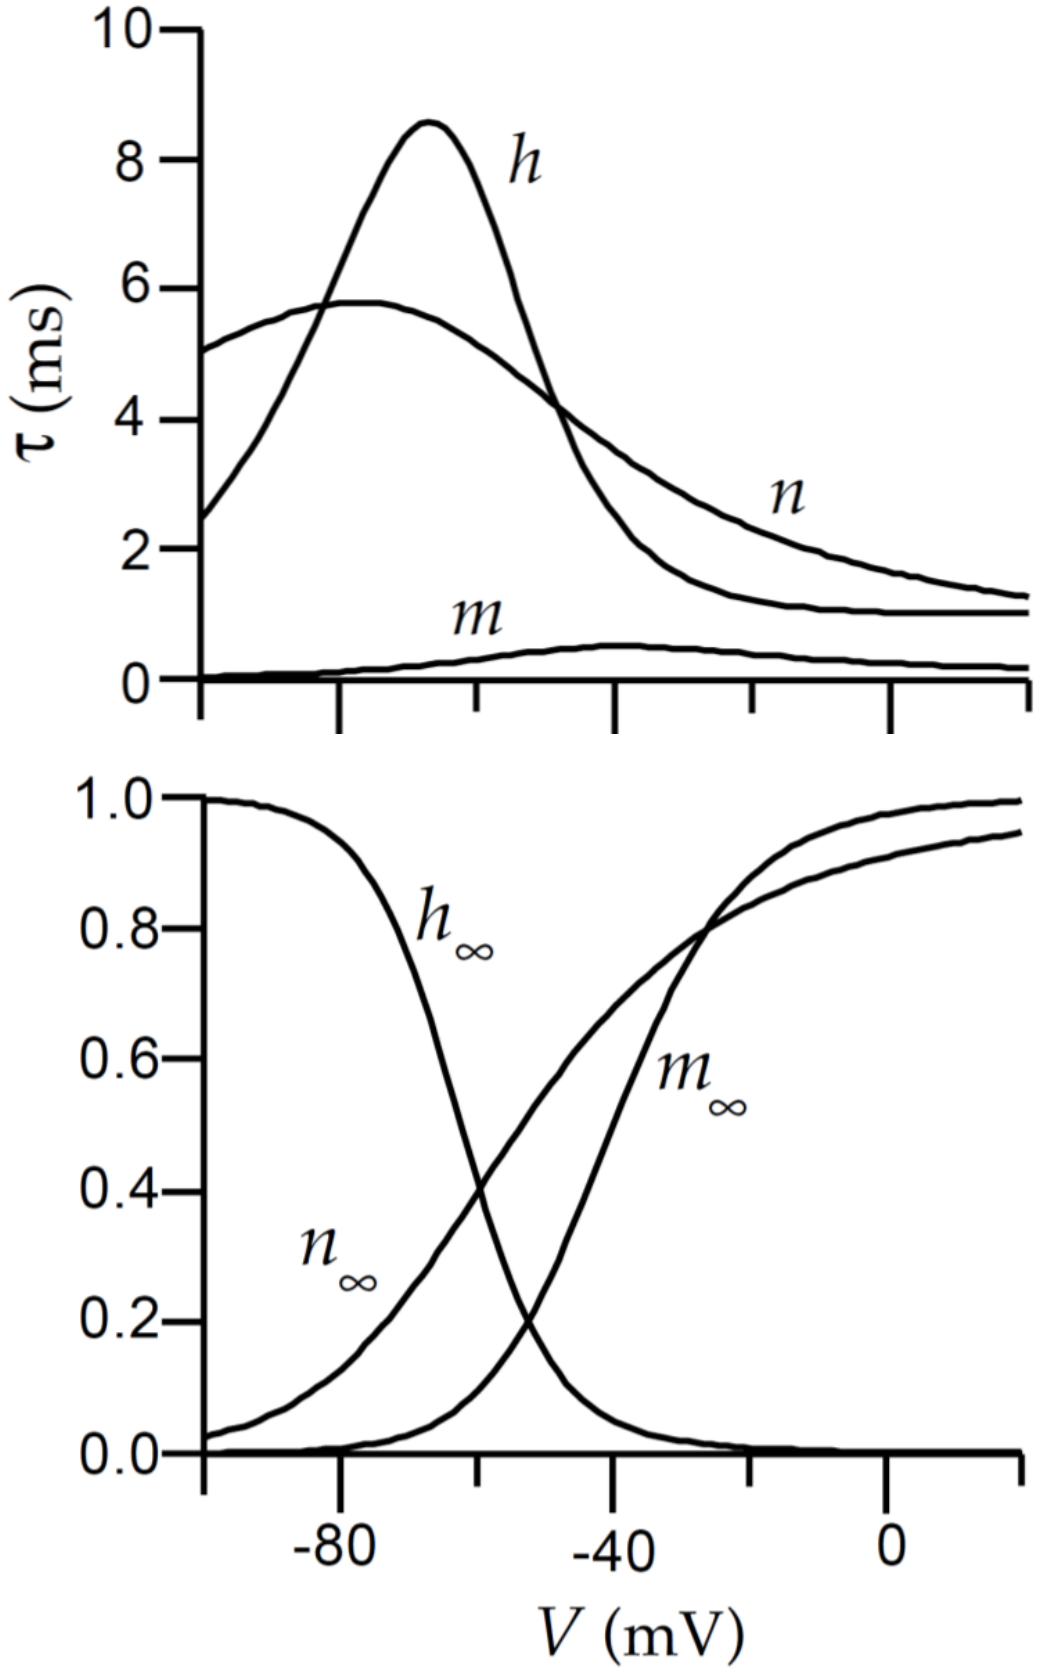
\includegraphics[scale=0.28]{05_4}
    \centering
\end{figure}
In the following it is instead shown what happens to the ionic currents (A), to the
membrane potential \(V_{m}\) (B), and to the gating particles respectively in two distinct
cases:
\begin{itemize}
    \item \textit{Solid} lines: the input current pulse overcomes the threhsold and generates
          an action potential (suprathreshold stimulus).
    \item \textit{Dashed} lines: the input current pulse is not high enough to produce an
          action potential (subthreshold stimulus).
\end{itemize}
\begin{figure}[H]
    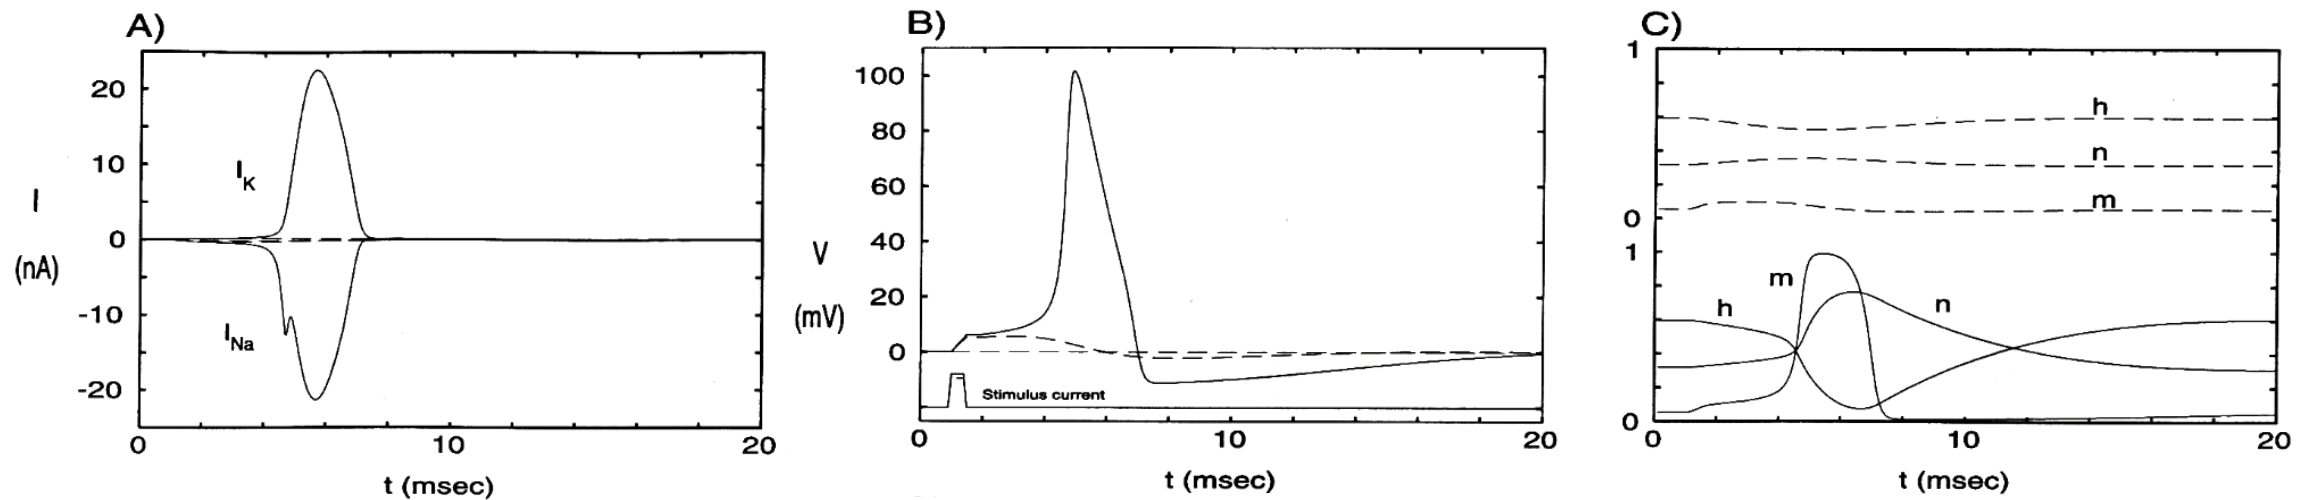
\includegraphics[scale=0.34]{05_5}
    \centering
\end{figure}
To sum up, the HH model is capable to:
\begin{itemize}
    \item Generate action potentials in a correct manner.
    \item Wait for a certain threshold to be overcome in order to initiate a spike.
    \item Exhibit a physiological refractory period after the firing of an action potential.
\end{itemize}
Lastly, it is important to highlight that the kinetics of channels, driven by \(\alpha\) and
\(\beta\) functions, are strongly dependent on temperature as well.

\subsection{Hodgkin-Huxley Model Dynamics}
As show in the picture below, the HH model is capable to fire an action potential
whenever the input stimulus overcomes a certain activation threshold. If this is not
the case, a passive potential - i.e., a partial depolarization - occurs. Note that
the action potential shape produced by this model is highly compatible with the one
observed in experiments.
\begin{figure}[H]
    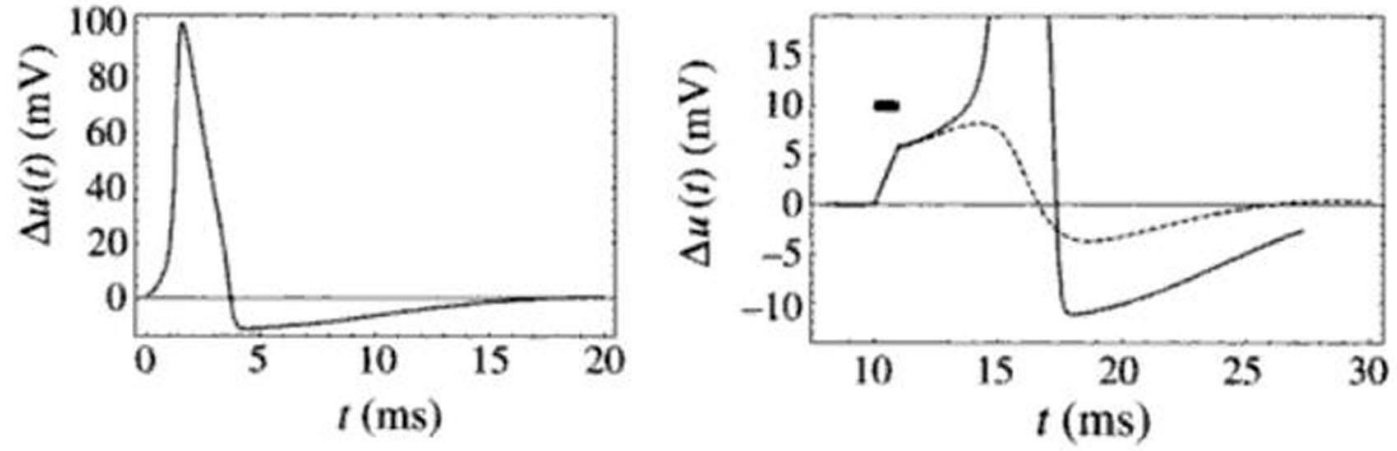
\includegraphics[scale=0.5]{05_6}
    \centering
\end{figure}
If a constant suprathreshold stimulation is provided, then a regular spike train is
observed. The spiking interval is \(T\) and is related to the stimulus amplitude, as
shown by the gain function on the right side. Note that the firing frequency \(f=T^{-1}\)
and it is dependent on the input current (as long as the threhsold is overcome). A minimum
firing rate (\(58\;Hz\)) is present, thus this model cannot fire at lower frequencies.
\begin{figure}[H]
    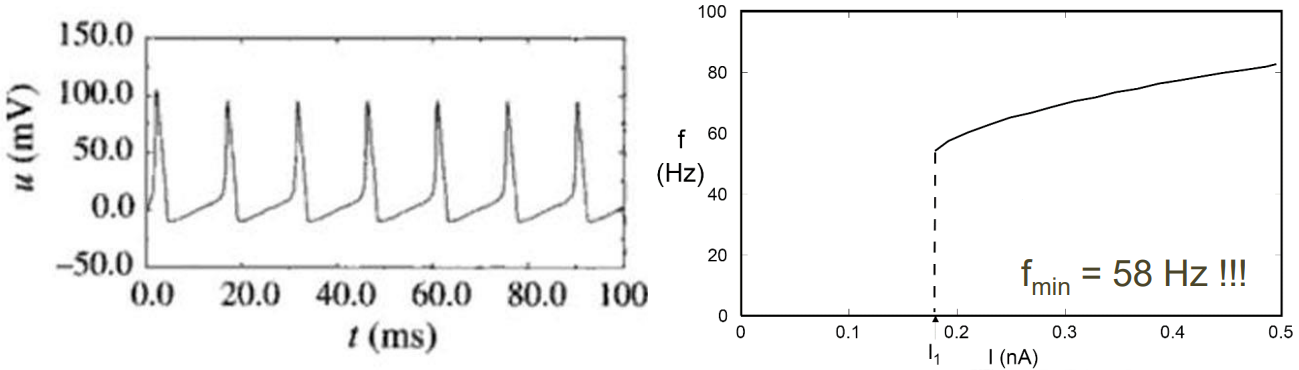
\includegraphics[scale=0.5]{05_7}
    \centering
\end{figure}
Note that if the input current is gradually increased, a higher applied current is needed
to elicit an action potential. In general, a fair current exploits the positive feedback
coming from the fact that Na\({}^{+}\) activating channels (\(m\)) are much faster than the
inactivating ones (\(h\)) and the K\({}^{+}\) activating channels (\(n\)). However, if the
membrane potential is incrementally raised (as the input current increases), the negative
feedback component has time to become stronger. In this condition the neuron is bistable:
\begin{itemize}
    \item Silent if initially quiescent.
    \item Sustained firing if it was already spiking.
\end{itemize}
If the provided stimulation is a step current, the model exhibits different behaviour
according to the size of the step \(\Delta{I}=I_{2}-I_{1}\) and to the final current \(I_{2}\).
\begin{itemize}
    \item Large \(\Delta{I}\Rightarrow\) Spike initiation is facilitated.
    \item Large \(I_{2}\Rightarrow\) Regular firing is more likely to occur.
\end{itemize}
\begin{figure}[H]
    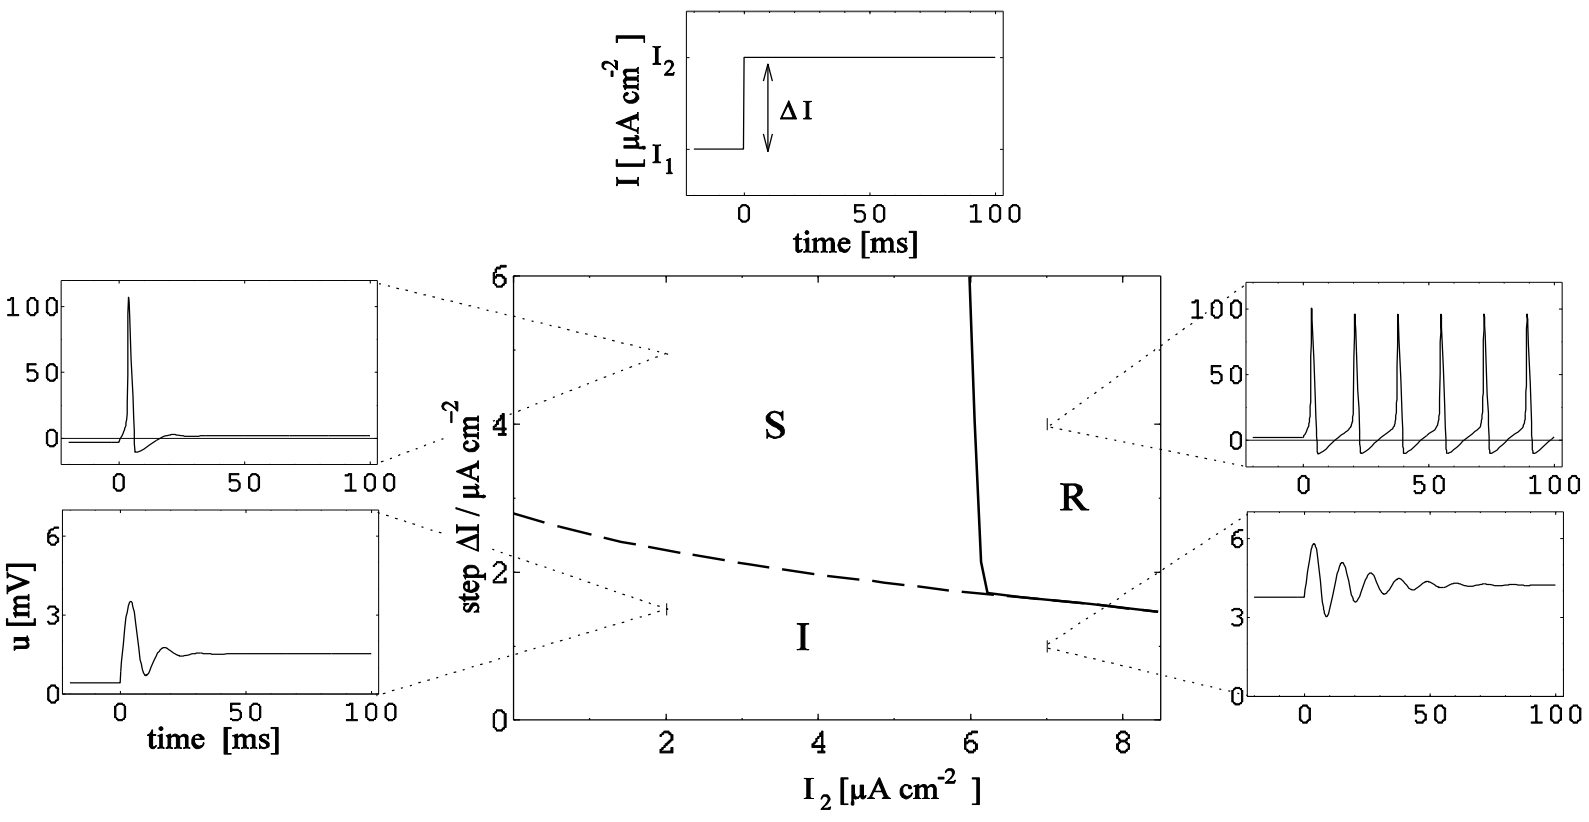
\includegraphics[scale=0.48]{05_8}
    \centering
\end{figure}
In general, the input stimuli can be either external, such as in the case of photoreceptors,
or coming from other close neurons; nonetheless, they are irregular and delivered in a
stochastic way. Typiclly, this means that the response of a neuron should be constituted of
irregual spikes superimposed on a generalized background activity, due to the presence of
noise.
\begin{figure}[H]
    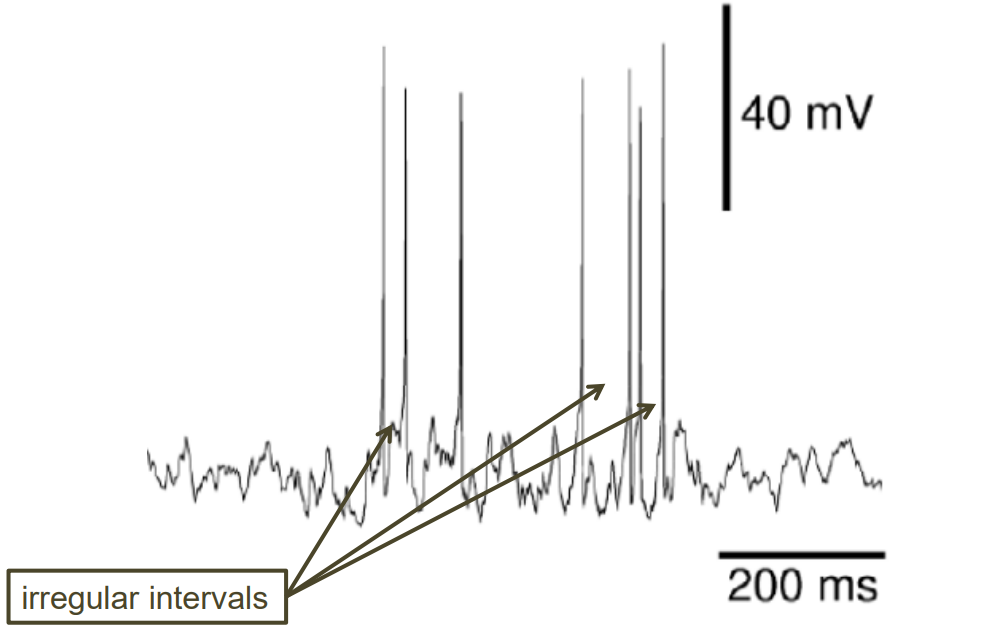
\includegraphics[scale=0.4]{05_9}
    \centering
\end{figure}

\subsection{Hodgkin-Huxley Model Limitations}
Hodgkin divided the neurons in three classes, according to their firing rate characteristics:
\begin{itemize}
    \item \textbf{Class I}: the firing frequency \(f\) can be arbitrarily low, depending on
          the amplitude of the input current. The magnitude of the input is encoded into the
          firing frequency.
    \item \textbf{Class II}: the firing rate is limted to a certain frequency band andd it is
          relatively insensitive to change in the input current magnitude.
    \item \textbf{Class III}: these neurons cannot exhibit sustained spiking activity.
\end{itemize}
The HH model works for Class II neurons, as shown by the gain function.
\begin{figure}[H]
    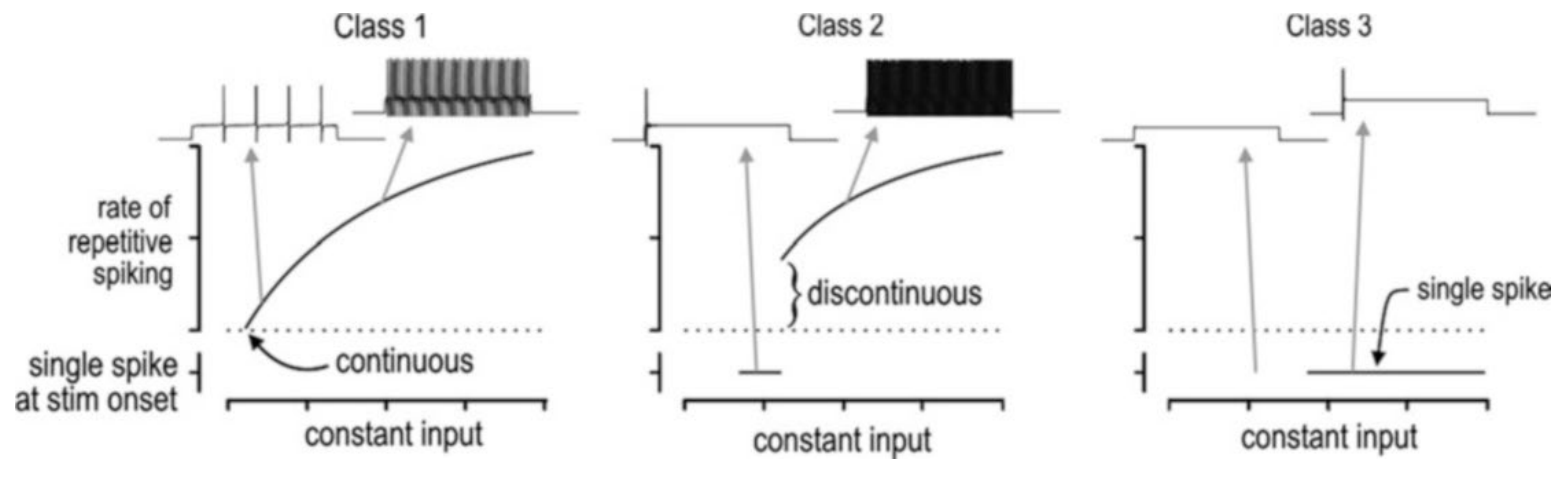
\includegraphics[scale=0.48]{05_10}
    \centering
\end{figure}
Therefore, the HH model does not work if the desired firing rate is low, as regular (tonic)
firing activity is elicited exclusively for high firing frequencies.\\
Another major drawback concerning the HH model is that it cannot reproduce all the
experimentally observed firing patterns. In particular, it is not suitable to model:
\begin{itemize}
    \item Bursting
    \item Adaptation
    \item Post-inhibitory rebound
    \item Resonator
\end{itemize}
Lastly, the HH model is based on the assumption that ion permeation processes are
both continuous and deterministic. Unluckily, this does not hold for very small patches of
cellular membrane, where channels are discrete; in addition, the opening and closing of
channels is ruled by stochastic processes and channels undergo random fluctuations between
open and closed stable states.
\begin{figure}[H]
    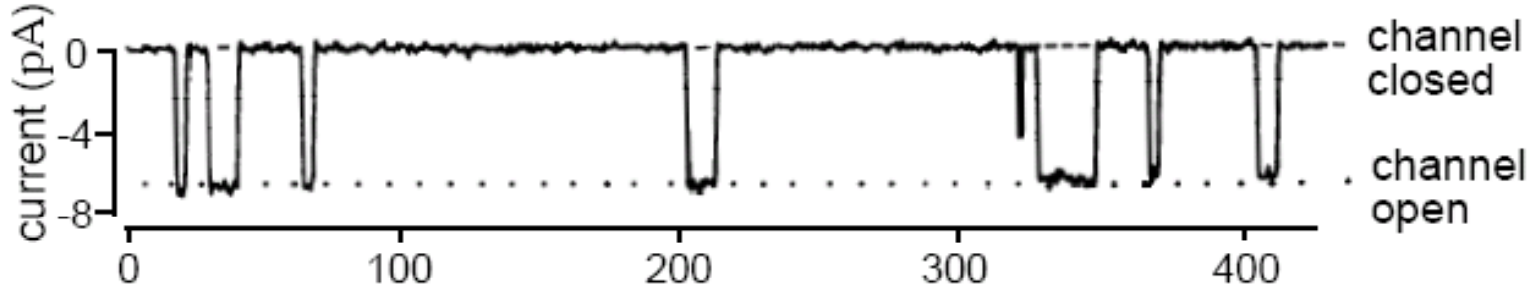
\includegraphics[scale=0.48]{05_11}
    \centering
\end{figure}